% This bring summarise and bring together all the previous section into a specification that should be fully expanded in the appendix with the following points, in providing what is known as the System Requirements Specification (SRS). This collects various information that you have previously agreed and worked on such as the UML diagrams.

\section{Purpose}
The main goal of this concept is to provide an exciting, and enjoyable experience for museum-goers through the use of AR. It includes users being lost, or searching for a specific location within the museum. The target audience is aware of this concept during the field research, it was discovered that the concept would make life easier for users and the museums since it would allow easy access to the information based on exhibitions.

\section{Scope}
This project will include creating an AR application for people to get an enjoyable journey in the museum. The project will be completed by 29 April 2019. The AR application will include simple navigation system to direct various part of the museum. Getting information on the user screen using the user's camera, and explore various museum using the app. 

\section{System Overview}
The application will perform all the basic tasks to help users with their journey in the museum. Such as navigating from point A to B, getting the user back on track in case they are lost, allowing the user to view information based on camera recognition of an exhibit.

\section{References}

\section{Definitions}

\section{Use Cases}
The use cases have been defined as follows:
\begin{enumerate}
    \item Use Case Model
    \item Activity Model
    \item User \& Acceptance Stories
    \begin{enumerate}
        \item In Exhibit going from A to B
        \item Getting information from an exhibition
        \item Exploring the museum
        \item User get lost in the museum
    \end{enumerate}
\end{enumerate}

\subsection{Use Case Model}
Two scenarios have been taken into account, where the user gets lost in the museum, and the user wants to explore the museum. When a user is lost, they need to enter their destination where the app will calculate their current location, and find the quickest route from the user's current position. The user follows that navigation until they arrive at their destination. For the exploration, the app will show the details where user know what they going to see in the museum.

\begin{figure}[H]
    \centering
    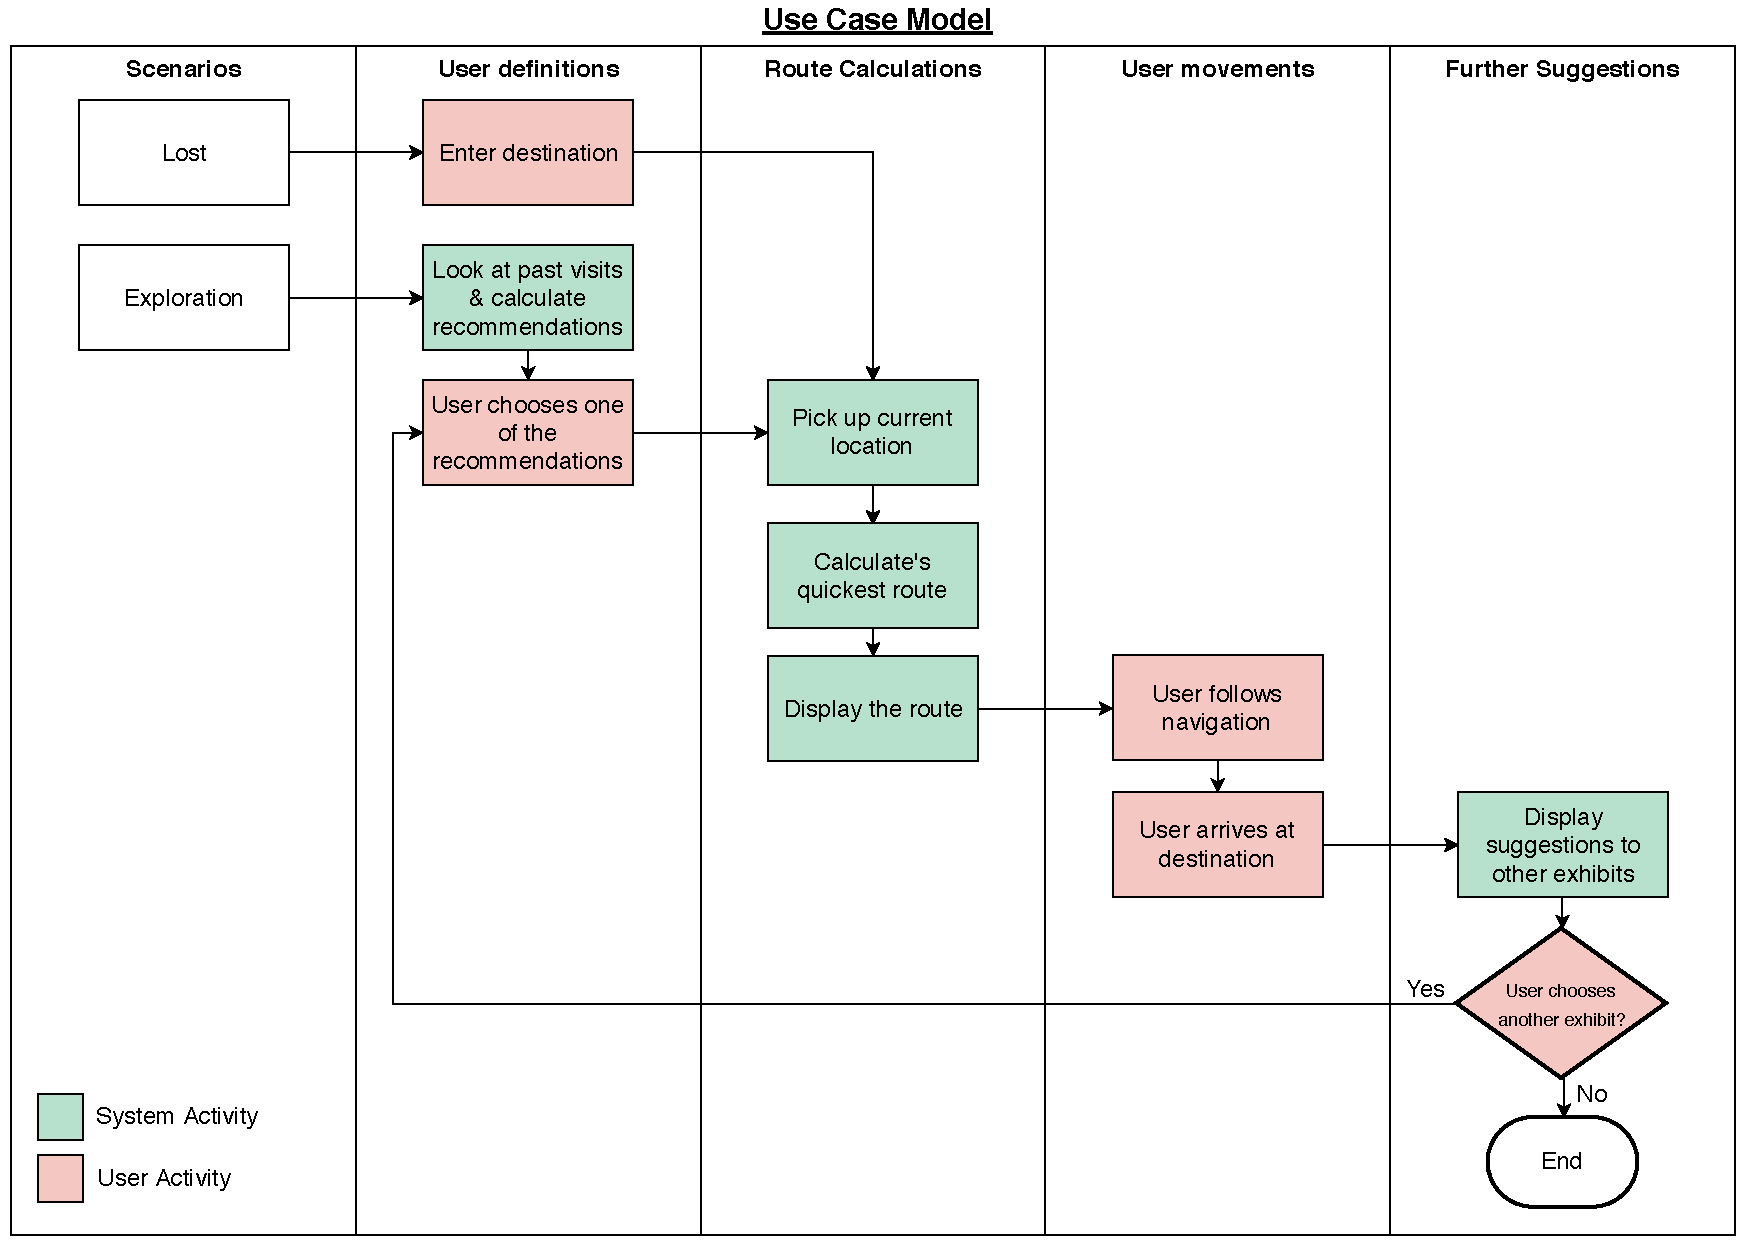
\includegraphics[width=\textwidth]
    {assets/use_case.pdf}
    \caption{Use Case Diagram}
    \label{fig:Use Case Diagram}
\end{figure}

\subsection{Activity Model}
This is based on the back-end of the application for example when the user searches about the museum, this history saved in the server where if the user wants to go to the same place then they can use our function called past visit.

\begin{figure}[H]
    \centering
    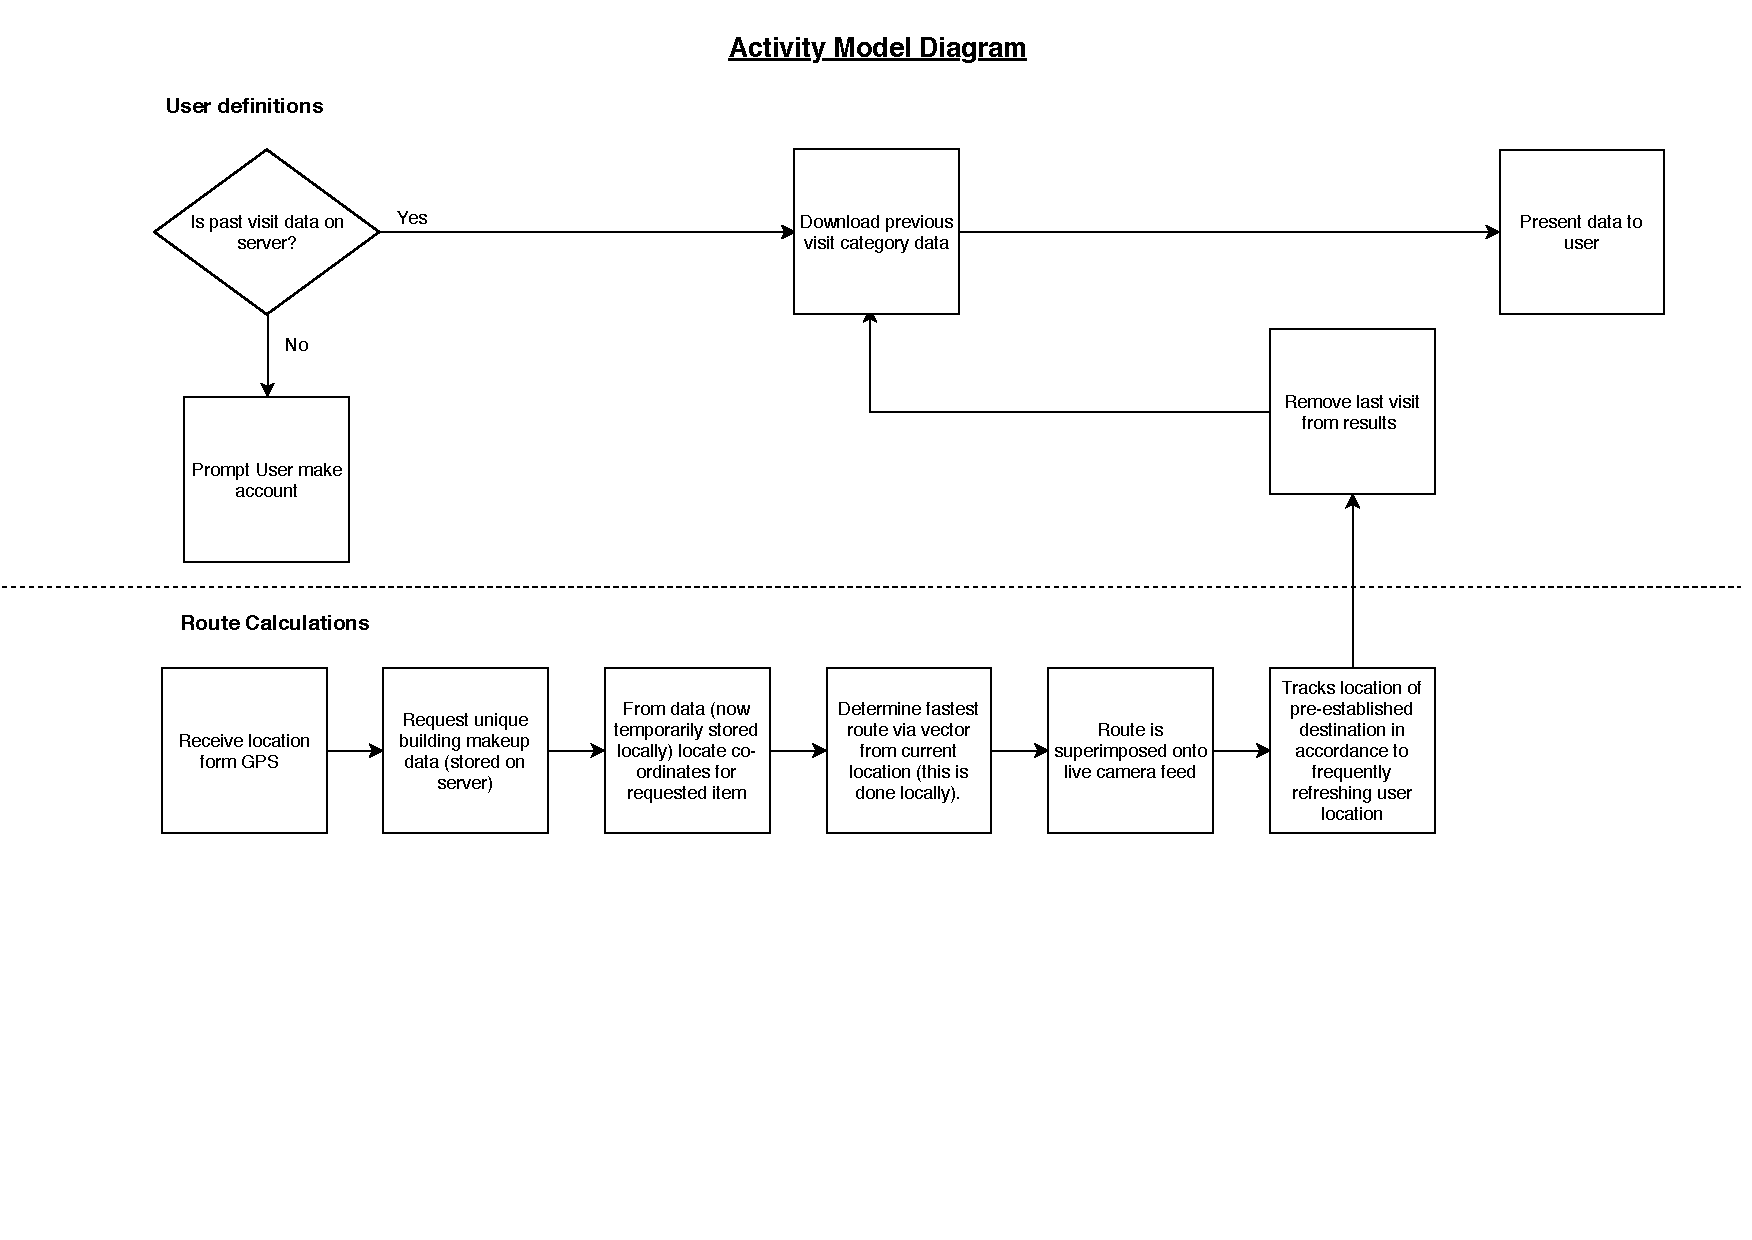
\includegraphics[angle=90, width=\textwidth]
    {assets/Activity_Diagram.pdf}
    \caption{Activity Model Diagram}
    \label{fig:Activity Model Diagram}
\end{figure}

\subsection{User \& Acceptance Stories}
This will describe what will be achieved once the application is ready to be used by the user. A diagram has been created based on different scenarios where it can be found if the application has achieved the user needs. 

\begin{figure}[H]
    \centering
    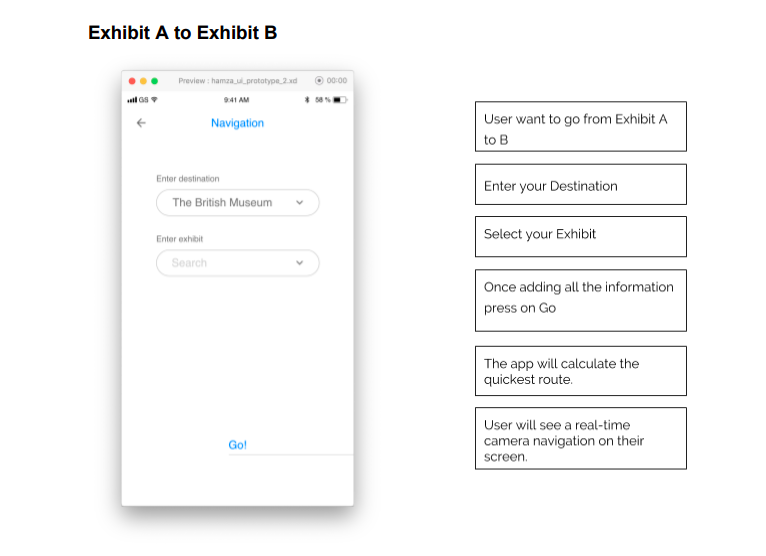
\includegraphics[width=\textwidth]
    {userstory_aTob.png}
    \caption{Going from point A to point B}
    \label{fig:AtoB}
\end{figure}

\begin{figure}[H]
    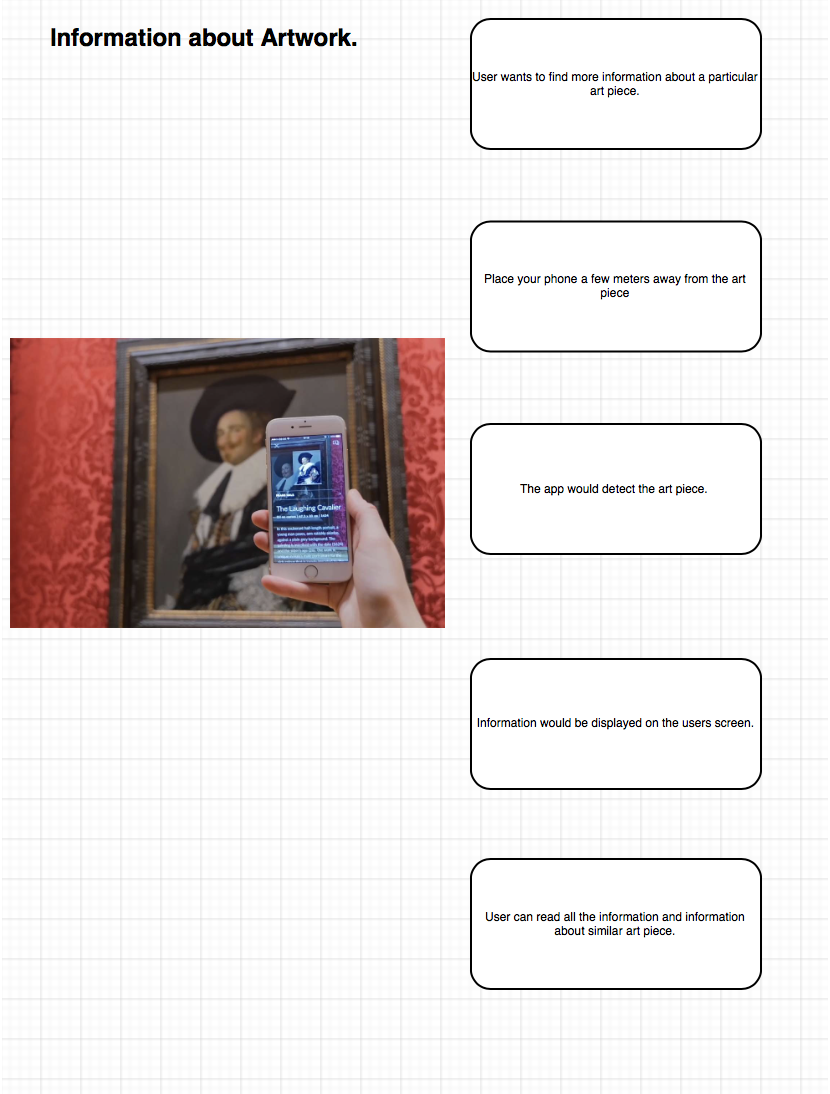
\includegraphics[width=\textwidth]
    {userstory_info.png}
    \caption{Getting information from exhibition}
    \label{fig:infofromexhibit}
\end{figure}

\begin{figure}[H]
    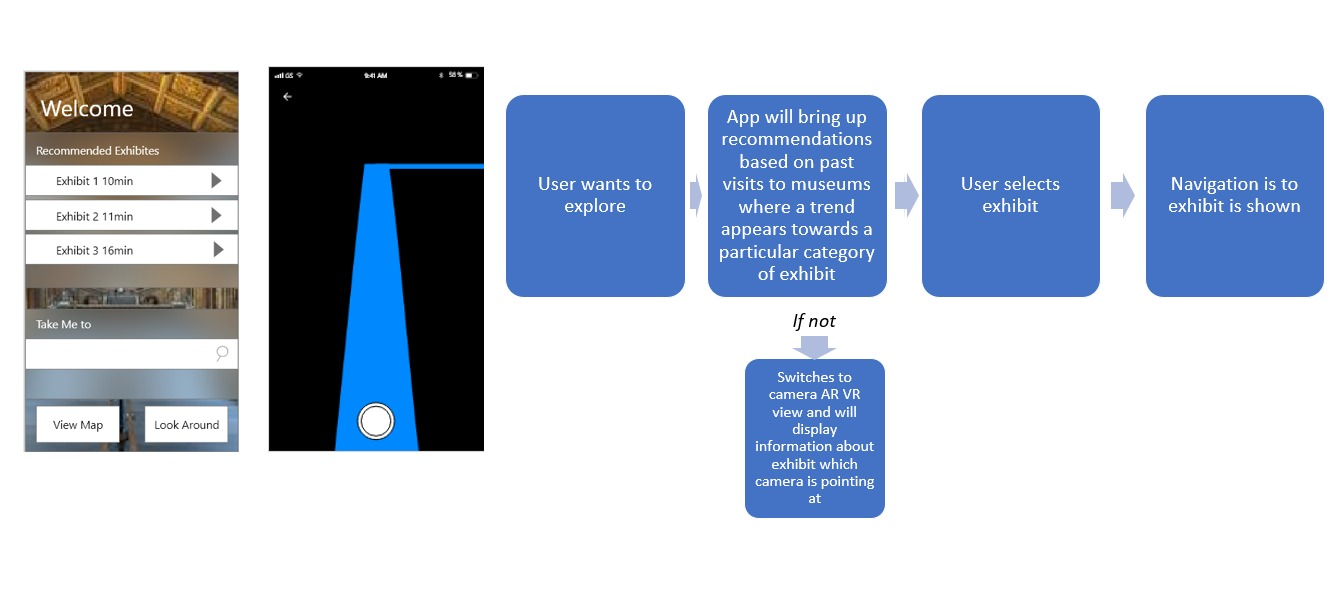
\includegraphics[width=\textwidth]
    {userstory_explore.jpeg}
    \caption{Exploring the museum}
    \label{fig:exploring}
\end{figure}

\section{Functional requirements}
\begin{itemize}
        \item Needs to be able to navigate the user to an exhibit through the use of AR.
        \item The app should be able to display navigational routes in real time.
        \item It should be able to calculate the quickest route to a destination.
        % \item Should be able to work in other museums
\end{itemize}

\section{Non-functional requirements}
% \begin{itemize}
        % \item Security is one of the most important parts of this project because the application stores username/passwords. The application will use MySQL to store data in the database and this will help to secure user data in the system.
% \end{itemize}
    